\documentclass[12pt,addpoints]{evalua}
\grado{2$^\circ$ de Secundaria}
\cicloescolar{2024-2025}
\materia{Matemáticas 2 \normalfont \color{darkgray} \small con adecuación curricular a \\Matemáticas 6$^\circ$ de Primaria.}
\unidad{2}
\title{Examen de la Unidad}
\aprendizajes{\tiny%
\item Expresa oralmente la sucesión numérica hasta billones, en español y hasta donde sea posible, en su lengua materna, de manera ascendente y descendente a partir de un número natural dado. Ordena, lee y escribe números naturales de más de nueve cifras e interpreta números decimales en diferentes contextos. Identifica semejanzas y diferencias entre el sistema de numeración decimal y otros sistemas como el maya y el romano\\[-1.5em]
	% \item Suma y resta, su relación como operaciones inversas.
	\item A partir de situaciones problemáticas vinculadas a diferentes contextos, suma y resta números decimales y fracciones con diferentes denominadores.\\[-1.5em]
	% \item Multiplicación y división, su relación como operaciones inversas.
	\item Resuelve situaciones problemáticas vinculadas a diferentes contextos que implican dividir números decimales entre naturales. También, dividir números fraccionarios entre números naturales.\\[-1.5em]
	% \item Relaciones de proporcionalidad.
	\item A partir de situaciones problemáticas de proporcionalidad vinculadas a diferentes contextos, determina valores faltantes en las que en ocasiones se conoce el valor unitario y en otras no.\\[-1.5em]
	% \item Ubicación espacial.
	\item Lee, interpreta y elabora planos para comunicar la ubicación de seres vivos y objetos.\\[-1.5em]
}
\author{Prof.: Julio César Melchor Pinto}
 \begin{document}%\vfill
% \afterpage{\blankpage}%
% % \begin{multicols}{2}
% 	\tableofcontents
% % \end{multicols}
% \newpage
\begin{questions}\large

   \addcontentsline{toc}{section}{Unidad 2}
	\section*{Unidad 2}

	\question[8]{Escribe sobre la línea el nombre que recibe cada figura geométrica de acuerdo con su número de lados:

\begin{multicols}{2}
	\begin{parts}
		\part 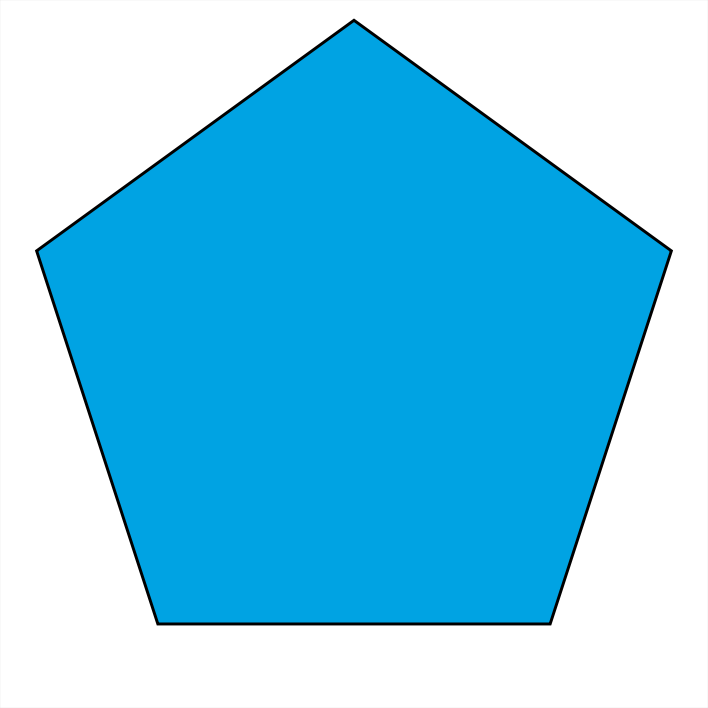
\includegraphics[width=75px]{../images/pentagono_azul.png}  \fillin[pentágono][0.75in]
		% \part 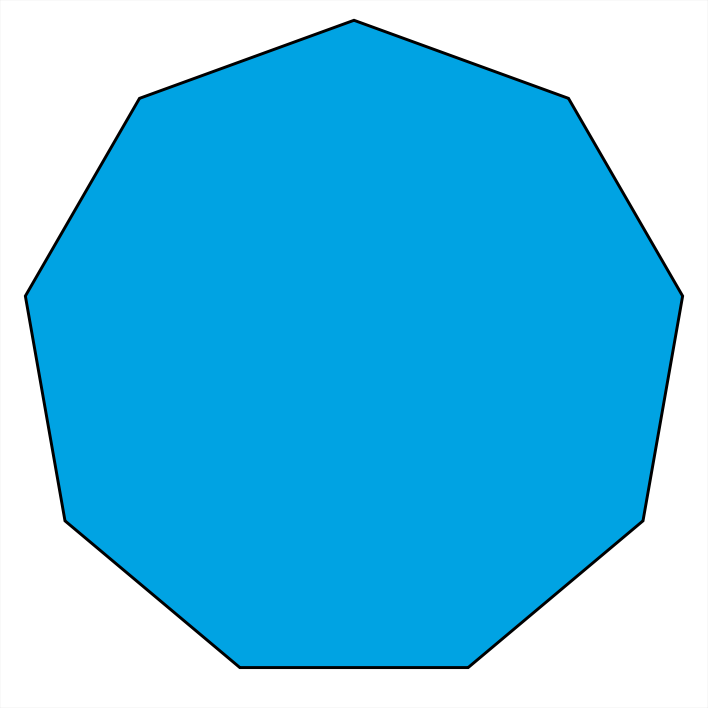
\includegraphics[width=75px]{../images/nonagono_azul.png}   \fillin[nonágono][0.75in]
		\part 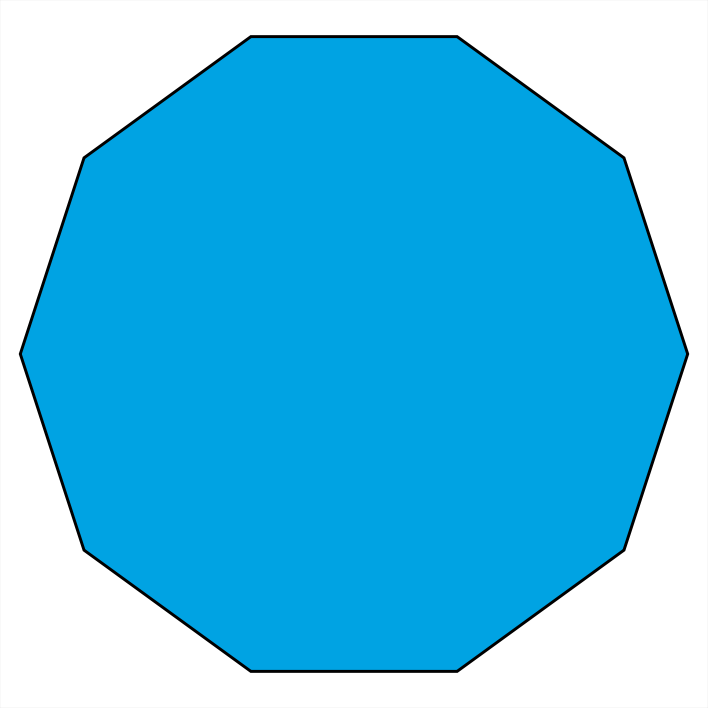
\includegraphics[width=75px]{../images/decagono_azul.png}   \fillin[decágono][0.75in]
		\part 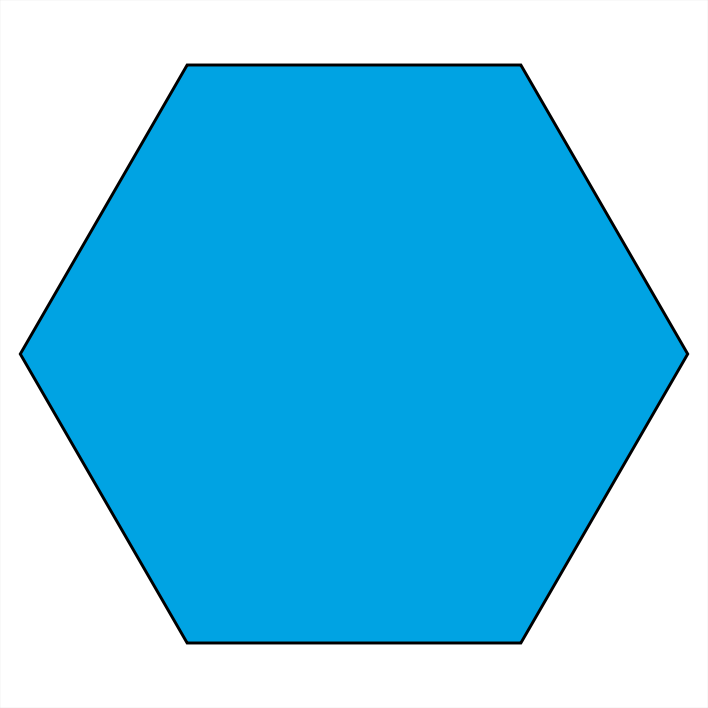
\includegraphics[width=75px]{../images/hexagono_azul.png}   \fillin[hexágono][0.75in]
		\part 
\includegraphics[width=100px]{../images/rectangulo_azul.png} \fillin[rectángulo][0.75in]
		% \part 
\includegraphics[width=75px]{../images/cuadrado_azul.png}   \fillin[cuadrado][0.75in]
	\end{parts}
\end{multicols}
}

\newpage

	\question[8]{Realiza las siguientes multiplicaciones:

	\begin{multicols}{2}
		\begin{parts}
			\part Multiplica $20\times800=$ \fillin[16000]
			\part Multiplica $60\times50=$ \fillin[3000]
			% \part Multiplica $900\times80=$ \fillin[172000]
			\part Multiplica $90\times700=$ \fillin[63000]
			\part Multiplica $100\times500=$ \fillin[50000]
			% \part Multiplica $120\times40=$ \fillin[4800]
			% \part Multiplica $200\times5000=$ \fillin[1000000]
			% \part Multiplica $5000\times20=$ \fillin[100000]
			% \part Multiplica $700\times50=$ \fillin[35000]
			% \part Multiplica $200\times20=$ \fillin[4000]
		\end{parts}
	\end{multicols}
}

\question[8]{Observa los siguientes \'angulos y estima la medida en cada inciso.

	\begin{multicols}{2}
		\begin{parts}
			\part
			\begin{minipage}{0.4\linewidth}
				\begin{figure}[H]
					\begin{center}
						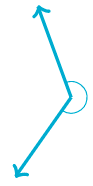
\includegraphics[width=0.5\textwidth]{../images/act003a12}
					\end{center}
					\caption{}
					\label{fig:act003a12}
				\end{figure}
			\end{minipage}
			\begin{minipage}{0.6\linewidth}
				\begin{choices}
					\choice 70
					\choice 85
					\choice 310
					\CorrectChoice 235
				\end{choices}
			\end{minipage}

			\part
			\begin{minipage}{0.4\linewidth}
				\begin{figure}[H]
					\begin{center}
						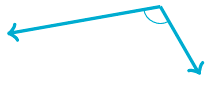
\includegraphics[width=0.8\textwidth]{../images/act003a13}
					\end{center}
					\caption{}
					\label{fig:act003a13}
				\end{figure}
			\end{minipage}
			\begin{minipage}{0.6\linewidth}
				\begin{choices}
					\choice 315
					\CorrectChoice 110
					\choice 240
					\choice 85
				\end{choices}
			\end{minipage}

			\part
			\begin{minipage}{0.4\linewidth}
				\begin{figure}[H]
					\begin{center}
						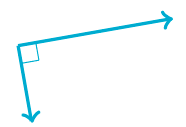
\includegraphics[width=0.8\textwidth]{../images/act003a14}
					\end{center}
					\caption{}
					\label{fig:act003a14}
				\end{figure}
			\end{minipage}
			\begin{minipage}{0.6\linewidth}
				\begin{choices}
					\choice 25
					\choice 220
					\CorrectChoice 90
					\choice 180
				\end{choices}
			\end{minipage}

			% \part
			% \begin{minipage}{0.4\linewidth}
			% 	\begin{figure}[H]
			% 		\begin{center}
			% 			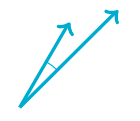
\includegraphics[width=0.8\textwidth]{../images/act003a15}
			% 		\end{center}
			% 		\caption{}
			% 		\label{fig:act003a15}
			% 	\end{figure}
			% \end{minipage}
			% \begin{minipage}{0.6\linewidth}
			% 	\begin{choices}
			% 		\choice 165
			% 		\choice 115
			% 		\choice 90
			% 		\CorrectChoice 15
			% 	\end{choices}
			% \end{minipage}

			\part
			\begin{minipage}{0.4\linewidth}
				\begin{figure}[H]
					\begin{center}
						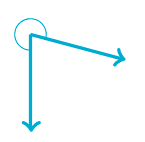
\includegraphics[width=0.8\textwidth]{../images/act003a16}
					\end{center}
					\caption{}
					\label{fig:act003a16}
				\end{figure}
			\end{minipage}
			\begin{minipage}{0.6\linewidth}
				\begin{choices}
					\choice 190
					\choice 40
					\choice 285
					\choice 100
				\end{choices}
			\end{minipage}

			% \part
			% \begin{minipage}{0.4\linewidth}
			% 	\begin{figure}[H]
			% 		\begin{center}
			% 			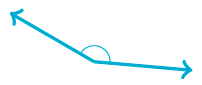
\includegraphics[width=0.8\textwidth]{../images/act003a17}
			% 		\end{center}
			% 		\caption{}
			% 		\label{fig:act003a17}
			% 	\end{figure}
			% \end{minipage}
			% \begin{minipage}{0.6\linewidth}
			% 	\begin{choices}
			% 		\choice 25
			% 		\choice 105
			% 		\choice 90
			% 		\CorrectChoice 155
			% 	\end{choices}
			% \end{minipage}

			% \part
			% \begin{minipage}{0.4\linewidth}
			% 	\begin{figure}[H]
			% 		\begin{center}
			% 			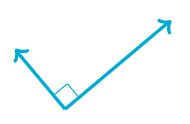
\includegraphics[width=0.8\textwidth]{../images/act003a18}
			% 		\end{center}
			% 		\caption{}
			% 		\label{fig:act003a18}
			% 	\end{figure}
			% \end{minipage}
			% \begin{minipage}{0.6\linewidth}
			% 	\begin{choices}
			% 		\CorrectChoice 90
			% 		\choice 125
			% 		\choice 360
			% 		\choice 60
			% 	\end{choices}
			% \end{minipage}

			% \part
			% \begin{minipage}{0.4\linewidth}
			% 	\begin{figure}[H]
			% 		\begin{center}
			% 			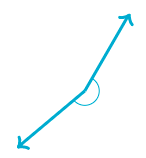
\includegraphics[width=0.8\textwidth]{../images/act003a19}
			% 		\end{center}
			% 		\caption{}
			% 		\label{fig:act003a19}
			% 	\end{figure}
			% \end{minipage}
			% \begin{minipage}{0.6\linewidth}
			% 	\begin{choices}
			% 		\choice 335
			% 		\choice 110
			% 		\CorrectChoice 200
			% 		\choice 50
			% 	\end{choices}
			% \end{minipage}

			% \part
			% \begin{minipage}{0.4\linewidth}
			% 	\begin{figure}[H]
			% 		\begin{center}
			% 			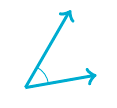
\includegraphics[width=0.8\textwidth]{../images/act003a20}
			% 		\end{center}
			% 		\caption{}
			% 		\label{fig:act003a20}
			% 	\end{figure}
			% \end{minipage}
			% \begin{minipage}{0.6\linewidth}
			% 	\begin{choices}
			% 		\CorrectChoice 50
			% 		\choice 110
			% 		\choice 15
			% 		\choice 95
			% 	\end{choices}
			% \end{minipage}


			% \part
			% \begin{minipage}{0.4\linewidth}
			% 	\begin{figure}[H]
			% 		\begin{center}
			% 			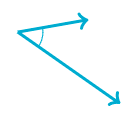
\includegraphics[width=0.8\textwidth]{../images/act003a21}
			% 		\end{center}
			% 		\caption{}
			% 		\label{fig:act003a21}
			% 	\end{figure}
			% \end{minipage}
			% \begin{minipage}{0.6\linewidth}
			% 	\begin{choices}
			% 		\CorrectChoice 45
			% 		\choice 75
			% 		\choice 120
			% 		\choice 150
			% 	\end{choices}
			% \end{minipage}

			% \part
			% \begin{minipage}{0.4\linewidth}
			% 	\begin{figure}[H]
			% 		\begin{center}
			% 			
\includegraphics[width=0.3\textwidth]{../images/act003a22}
			% 		\end{center}
			% 		\caption{}
			% 		\label{fig:act003a22}
			% 	\end{figure}
			% \end{minipage}
			% \begin{minipage}{0.6\linewidth}
			% 	\begin{choices}
			% 		\choice 55
			% 		\choice 95
			% 		\choice 185
			% 		\CorrectChoice 150
			% 	\end{choices}
			% \end{minipage}

			% \part
			% \begin{minipage}{0.4\linewidth}
			% 	\begin{figure}[H]
			% 		\begin{center}
			% 			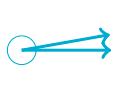
\includegraphics[width=0.35\textwidth]{../images/act003a23}
			% 		\end{center}
			% 		\caption{}
			% 		\label{fig:act003a23}
			% 	\end{figure}
			% \end{minipage}
			% \begin{minipage}{0.6\linewidth}
			% 	\begin{choices}
			% 		\choice 190
			% 		\CorrectChoice 350
			% 		\choice 290
			% 		\choice 300
			% 	\end{choices}
			% \end{minipage}

			% \part
			% \begin{minipage}{0.4\linewidth}
			% 	\begin{figure}[H]
			% 		\begin{center}
			% 			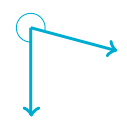
\includegraphics[width=0.35\textwidth]{../images/act003a24}
			% 		\end{center}
			% 		\caption{}
			% 		\label{fig:act003a24}
			% 	\end{figure}
			% \end{minipage}
			% \begin{minipage}{0.6\linewidth}
			% 	\begin{choices}
			% 		\choice 260
			% 		\CorrectChoice 285
			% 		\choice 320
			% 		\choice 190
			% 	\end{choices}
			% \end{minipage}

			% \part
			% \begin{minipage}{0.4\linewidth}
			% 	\begin{figure}[H]
			% 		\begin{center}
			% 			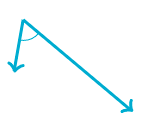
\includegraphics[width=0.35\textwidth]{../images/act003a25}
			% 		\end{center}
			% 		\caption{}
			% 		\label{fig:act003a25}
			% 	\end{figure}
			% \end{minipage}
			% \begin{minipage}{0.6\linewidth}
			% 	\begin{choices}
			% 		\choice 85
			% 		\choice 45
			% 		\CorrectChoice 60
			% 		\choice 135
			% 	\end{choices}
			% \end{minipage}

			% \part
			% \begin{minipage}{0.4\linewidth}
			% 	\begin{figure}[H]
			% 		\begin{center}
			% 			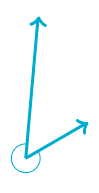
\includegraphics[width=0.3\textwidth]{../images/act003a26}
			% 		\end{center}
			% 		\caption{}
			% 		\label{fig:act003a26}
			% 	\end{figure}
			% \end{minipage}
			% \begin{minipage}{0.6\linewidth}
			% 	\begin{choices}
			% 		\choice 155
			% 		\CorrectChoice 305
			% 		\choice 295
			% 		\choice 355
			% 	\end{choices}
			% \end{minipage}

			% \part
			% \begin{minipage}{0.4\linewidth}
			% 	\begin{figure}[H]
			% 		\begin{center}
			% 			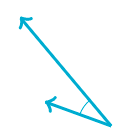
\includegraphics[width=0.35\textwidth]{../images/act003a27}
			% 		\end{center}
			% 		\caption{}
			% 		\label{fig:act003a27}
			% 	\end{figure}
			% \end{minipage}
			% \begin{minipage}{0.6\linewidth}
			% 	\begin{choices}
			% 		\CorrectChoice 30
			% 		\choice 130
			% 		\choice 80
			% 		\choice 5
			% 	\end{choices}
			% \end{minipage}

		\end{parts}
	\end{multicols}
}




\question[8]{Selecciona la opci\'on que responde a cada una de las preguntas de forma correcta.

	\begin{multicols}{2}
		\begin{parts}
			% \part Si un \'angulo mide $30^\circ$, es un \'angulo:

			% \begin{oneparchoices}
			% 	\CorrectChoice agudo
			% 	\choice recto
			% 	\choice obtuso
			% 	\choice llano
			% \end{oneparchoices}

			\part Si un \'angulo mide $29^\circ$, es un \'angulo:

			\begin{oneparchoices}
				\CorrectChoice agudo
				\choice recto
				\choice obtuso
				\choice llano
			\end{oneparchoices}

			\part Si un \'angulo mide $167^\circ$, es un \'angulo:

			\begin{oneparchoices}
				\choice agudo
				\choice recto
				\CorrectChoice obtuso
				\choice llano
			\end{oneparchoices}

			\part Si un \'angulo mide $45^\circ$, es un \'angulo:

			\begin{oneparchoices}
				\CorrectChoice agudo
				\choice recto
				\choice obtuso
				\choice llano
			\end{oneparchoices}
			\part Si un \'angulo mide $180^\circ$, es un \'angulo:

			\begin{oneparchoices}
				\choice agudo
				\choice recto
				\choice obtuso
				\CorrectChoice llano
			\end{oneparchoices}

			\part Si un \'angulo mide $90^\circ$, es un \'angulo:

			\begin{oneparchoices}
				\choice agudo
				\CorrectChoice recto
				\choice obtuso
				\choice llano
			\end{oneparchoices}

			\part Si un \'angulo mide $91^\circ$, es un \'angulo:

			\begin{oneparchoices}
				\choice agudo
				\choice recto
				\CorrectChoice obtuso
				\choice llano
			\end{oneparchoices}

			\part Si un \'angulo mide $10^\circ$, es un \'angulo:

			\begin{oneparchoices}
				\CorrectChoice agudo
				\choice recto
				\choice obtuso
				\choice llano
			\end{oneparchoices}

			\part Si un \'angulo mide $65^\circ$, es un \'angulo:

			\begin{oneparchoices}
				\CorrectChoice agudo
				\choice recto
				\choice obtuso
				\choice llano
			\end{oneparchoices}
			% \part Si un \'angulo mide $80^\circ$, es un \'angulo:

			% \begin{oneparchoices}
			% 	\CorrectChoice agudo
			% 	\choice recto
			% 	\choice obtuso
			% 	\choice llano
			% \end{oneparchoices}
		\end{parts}
	\end{multicols}
}

\question[4]{Convierte los siguientes números decimales a una fracción:

	\begin{multicols}{4}
		\begin{parts}
			% \part $0.248=$ \fillin[\fbox{$\dfrac{31}{125}$}][0cm]
			\part $0.46=$  \fillin[\fbox{$\dfrac{23}{50}$}][0cm]
			\part $0.24=$  \fillin[\fbox{$\dfrac{6}{25}$}][0cm]
			\part $0.9=$   \fillin[\fbox{$\dfrac{9}{10}$}][0cm]
			% \part $0.115=$ \fillin[\fbox{$\dfrac{23}{200}$}][0cm]
			% \part $0.66=$  \fillin[\fbox{$\dfrac{33}{50}$}][0cm]
			% \part $0.56=$  \fillin[\fbox{$\dfrac{14}{25}$}][0cm]
			\part $0.58=$  \fillin[\fbox{$\dfrac{29}{50}$}][0cm]
		\end{parts}
	\end{multicols}
}


\newpage



% \question[10]{Selecciona la opci\'on que responde a cada una de las preguntas de forma correcta.

% 		\begin{parts}
% 			\part Nuha pasaba por una puerta giratoria que debe rotar $160^\circ$ para permitirle el paso.
% 			El viento empujó la puerta alrededor de $40^\circ$. Nuha debe empujar el resto.

% 			\textbf{¿Cuál ecuación nos dará la medida del ángulo adicional a que Nuha debe empujar para poder salir?}

% 			\begin{choices}
% 				\choice $160 \div 40=a$
% 				\choice $160 + 40 = a$
% 				\choice $40 \times 2 = a$
% 				\choice $160 - 40 = a$
% 			\end{choices}

% 			\part ¿Cuál recta numérica representa mejor $8\times8$?
% 			\begin{choices}
% 				\choice 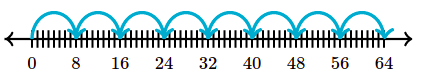
\includegraphics[width=0.5\textwidth]{../images/act003a01}
% 				\choice 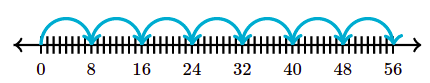
\includegraphics[width=0.5\textwidth]{../images/act003a02}
% 				\choice 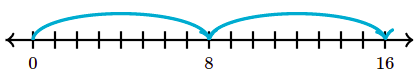
\includegraphics[width=0.5\textwidth]{../images/act003a03}
% 				\choice Ninguna de las anteriores.
% 			\end{choices}
% 		\end{parts}
% }

\question[10]{Resuelve los siguientes problemas sobre sumas y restas:

	\begin{multicols}{2}
		\begin{parts}
			

			\part Jorge está armando un rompecabezas de 500 piezas, si ha puesto 233 piezas, ¿cuántas piezas le faltan por poner a Jorge?

			\begin{solutionbox}{1cm}
				\opsub[style=text]{500}{233}
			\end{solutionbox}

			\part Carlos mide 183 centímetros y es 8 centímetros más alto que Julio, ¿cuántos centímetros mide Julio?

			\begin{solutionbox}{1cm}
				\opsub[style=text]{183}{8}
			\end{solutionbox}
		\end{parts}
	\end{multicols}
}

\question[10]{Clasifica las siguientes fracciones en propias, impropias o mixtas:

\begin{multicols}{5}
	\begin{parts}
		\part $\dfrac{5}{6}$   \fillin[Propia][0.5in]     \\[0.5em]
		\part $5\dfrac{5}{11}$ \fillin[Mixta][0.5in]      \\[0.5em]
		\part $\dfrac{13}{12}$   \fillin[Impropia][0.5in] \\[0.5em]
		\part $1\dfrac{2}{15}$  \fillin[Mixta][0.5in]     \\[0.5em]
		\part $\dfrac{42}{43}$   \fillin[Propia][0.5in]   \\[0.5em]
		\part $\dfrac{16}{9}$   \fillin[Impropia][0.5in]  \\[0.5em]
		\part $\dfrac{7}{3}$   \fillin[Impropia][0.5in]   \\[0.5em]
		\part $3\dfrac{2}{9}$  \fillin[Mixta][0.5in]      \\[0.5em]
		\part $\dfrac{3}{2}$   \fillin[Impropia][0.5in]   \\[0.5em]
		\part $1\dfrac{2}{3}$  \fillin[Mixta][0.5in]      \\[0.5em]
		% \part $\dfrac{7}{8}$   \fillin[Propia][0.5in]     \\[0.5em]
		% \part $\dfrac{6}{5}$   \fillin[Impropia][0.5in]   \\[0.5em]
	\end{parts}
\end{multicols}
}

\question[10]{Escribe sobre la línea el símbolo de mayor que ($>$), menor que ($<$), o igual ($=$) según corresponda.

	\begin{multicols}{5}
		\begin{parts}
			\part $\dfrac{2}{5}$ \fillin[$>$][0.3in] $\dfrac{1}{3}$\\[0.25em]
			\part $\dfrac{3}{4}$ \fillin[$<$][0.3in] $\dfrac{4}{5}$\\[0.25em]
			\part $\dfrac{2}{5}$ \fillin[$<$][0.3in] $\dfrac{2}{3}$\\[0.25em]
			\part $\dfrac{3}{2}$ \fillin[$=$][0.3in] $\dfrac{9}{6}$\\[0.25em]
			\part $\dfrac{5}{6}$ \fillin[$>$][0.3in] $\dfrac{4}{6}$\\[0.25em]
			\part $\dfrac{4}{3}$ \fillin[$>$][0.3in] $\dfrac{5}{4}$\\[0.25em]
			\part $\dfrac{1}{3}$ \fillin[$=$][0.3in] $\dfrac{9}{3}$\\[0.25em]
			\part $\dfrac{2}{3}$ \fillin[$<$][0.3in] $\dfrac{3}{2}$\\[0.25em]
			\part $\dfrac{3}{4}$ \fillin[$>$][0.3in] $\dfrac{2}{3}$\\[0.25em]
			\part $\dfrac{5}{6}$ \fillin[$>$][0.3in] $\dfrac{4}{5}$\\[0.25em]
		\end{parts}
	\end{multicols}
}


\question[10]{Escribe sobre la línea la fracción que representa cada imagen:

	\begin{multicols}{5}
		\begin{parts}
			\part 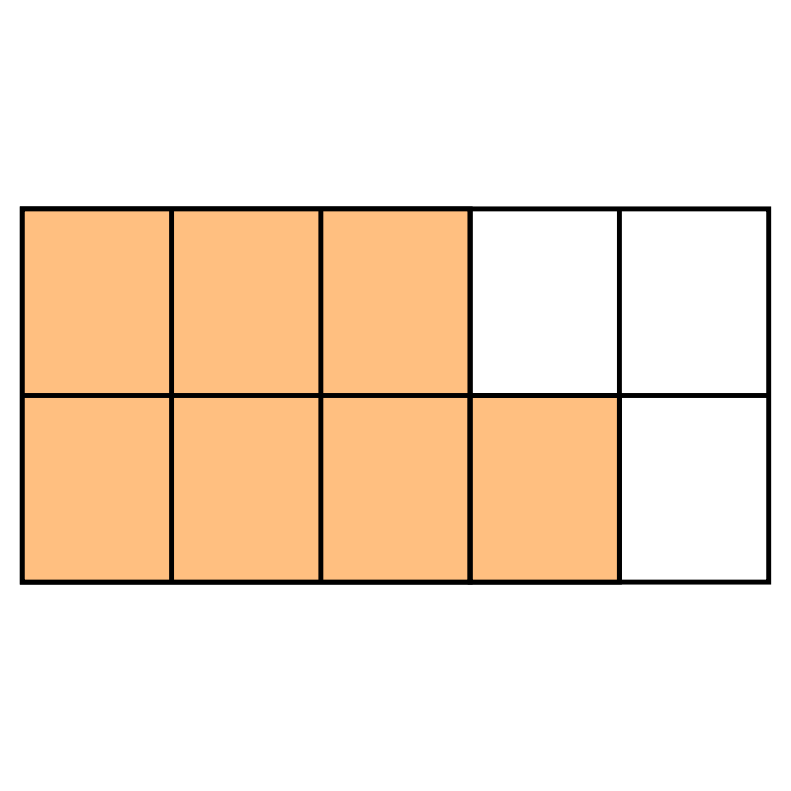
\includegraphics[width=60px]{../images/imagen_frac_5prim_7|10.png} \fillin[\fbox{$\dfrac{7}{10}$}][0in] \\[-0.5em]
			\part 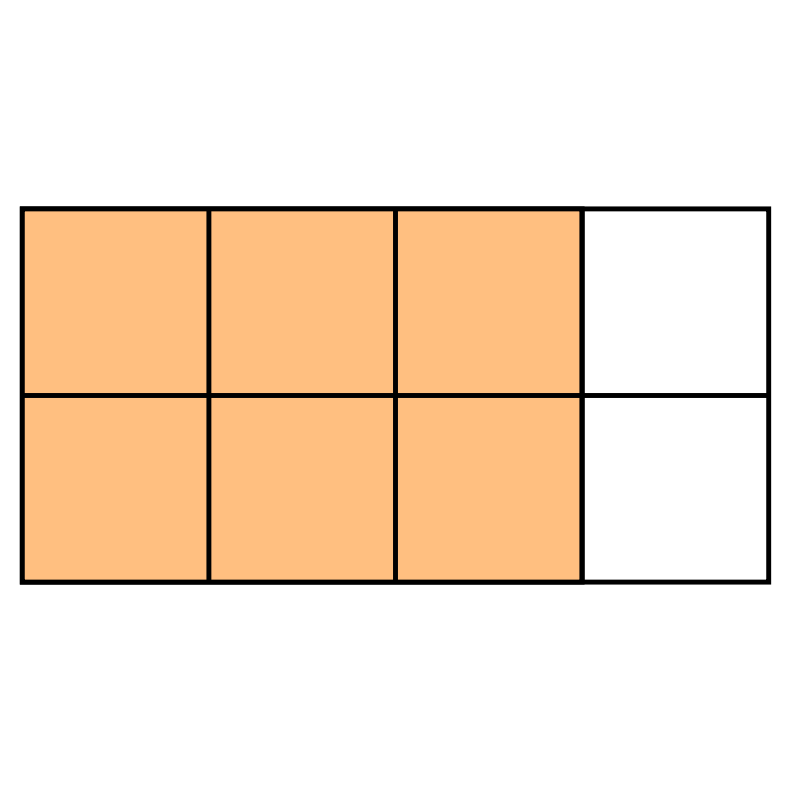
\includegraphics[width=60px]{../images/imagen_frac_5prim_6|8.png} \fillin[\fbox{$\dfrac{6}{8}$}][0in] \\[-0.5em]
			\part 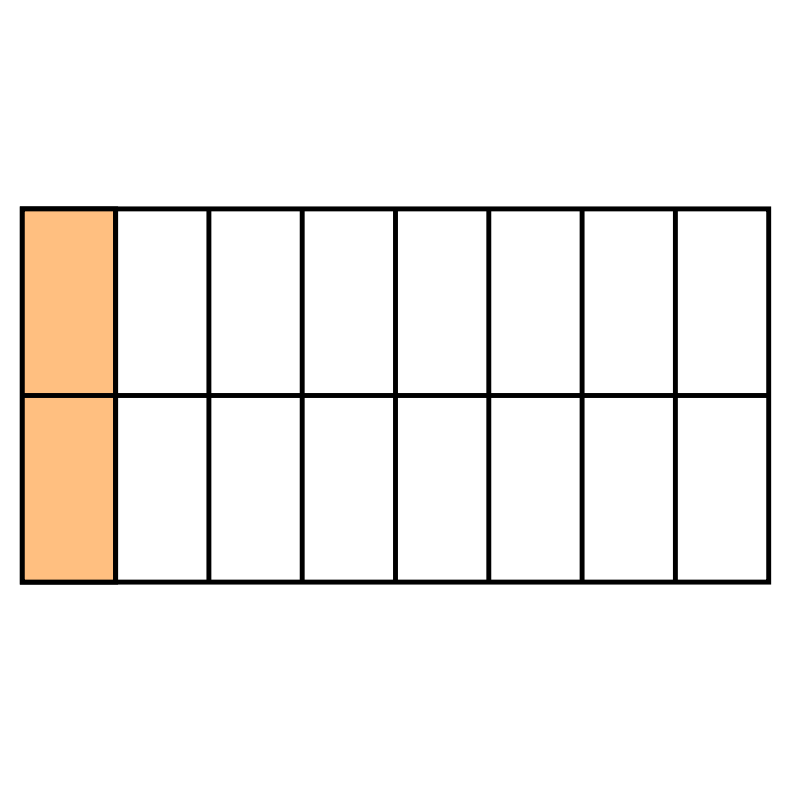
\includegraphics[width=60px]{../images/imagen_frac_5prim_2|16.png} \fillin[\fbox{$\dfrac{2}{16}$}][0in] \\[-0.5em]
			% \part 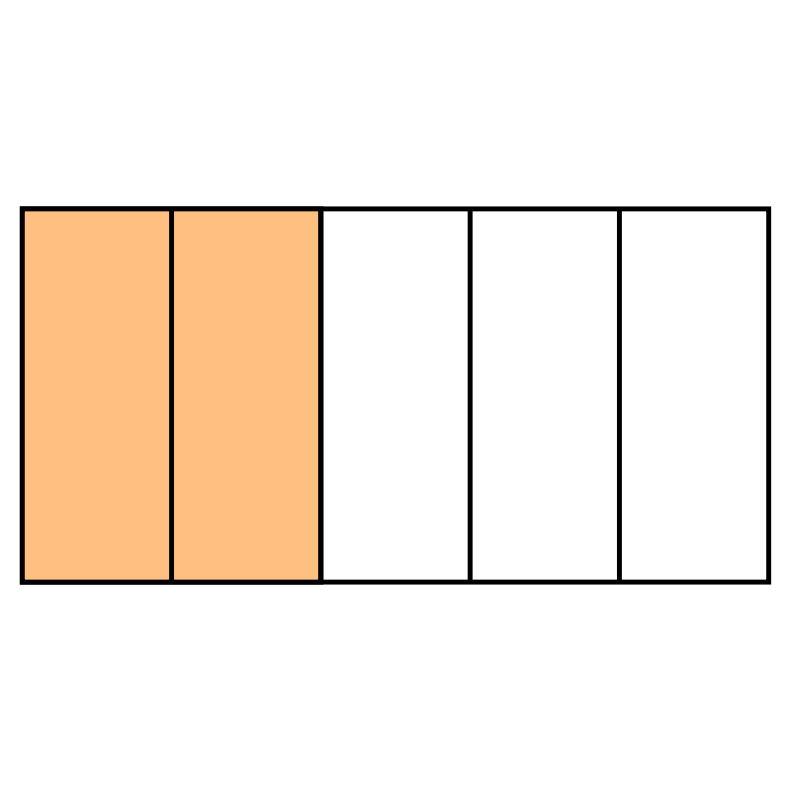
\includegraphics[width=60px]{../images/imagen_frac_5prim_2|5.png} \fillin[\fbox{$\dfrac{2}{5}$}][0in] \\[-0.5em]
			\part 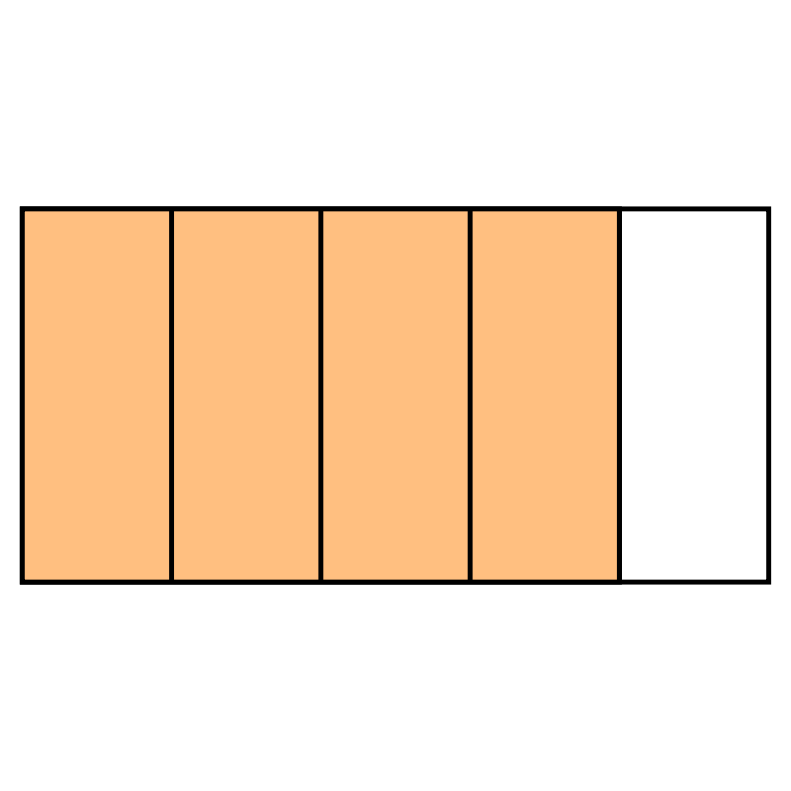
\includegraphics[width=60px]{../images/imagen_frac_5prim_4|5.png} \fillin[\fbox{$\dfrac{4}{5}$}][0in] \\[-0.5em]
			% \part 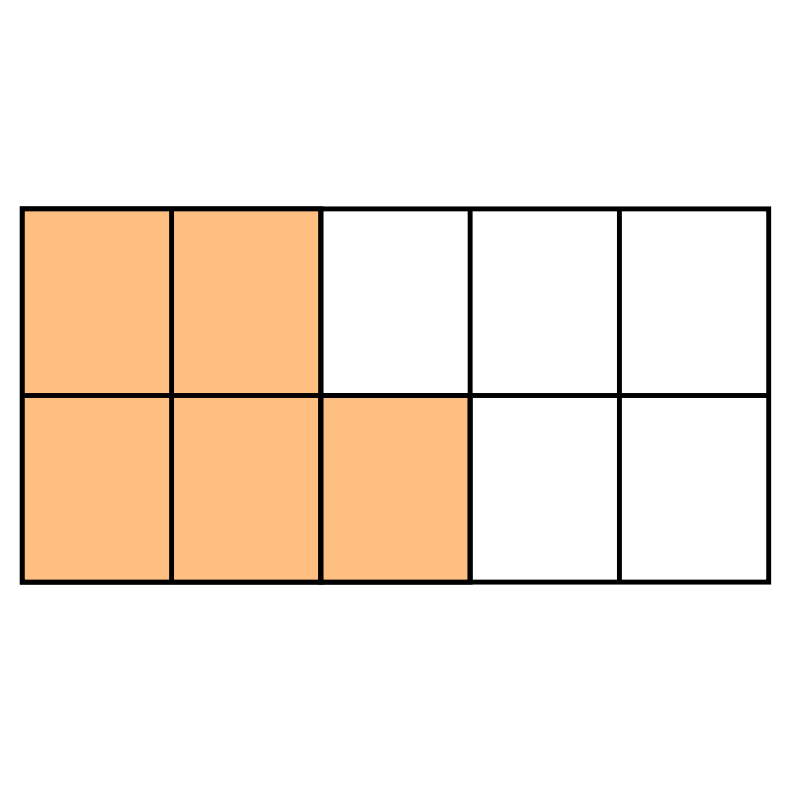
\includegraphics[width=60px]{../images/imagen_frac_5prim_5|10.png} \fillin[\fbox{$\dfrac{5}{10}$}][0in] \\[-0.5em]
			\part 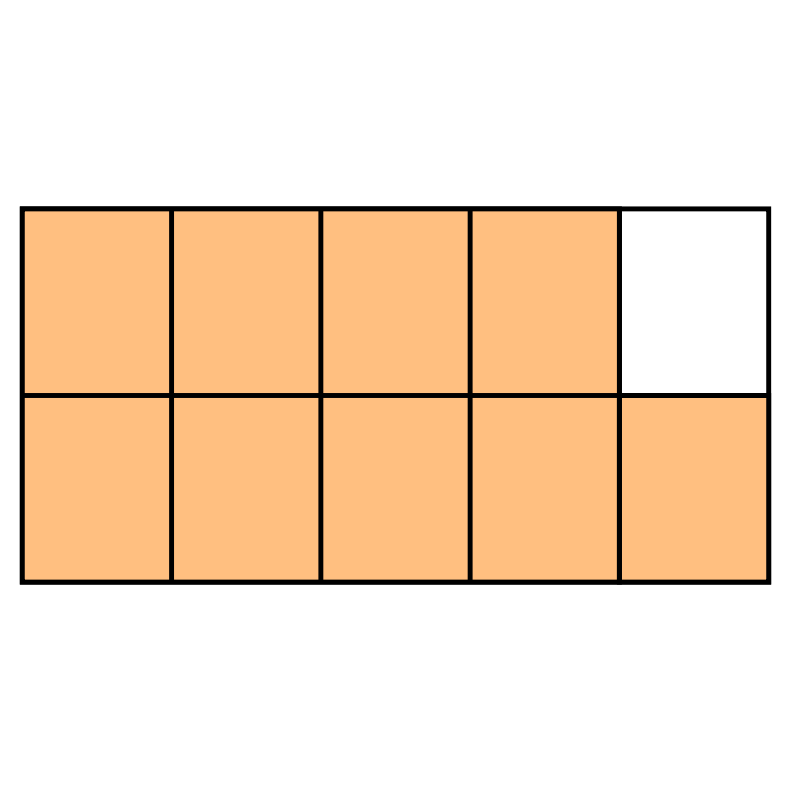
\includegraphics[width=60px]{../images/imagen_frac_5prim_9|10.png} \fillin[\fbox{$\dfrac{9}{10}$}][0in] \\[-0.5em]
			% \part 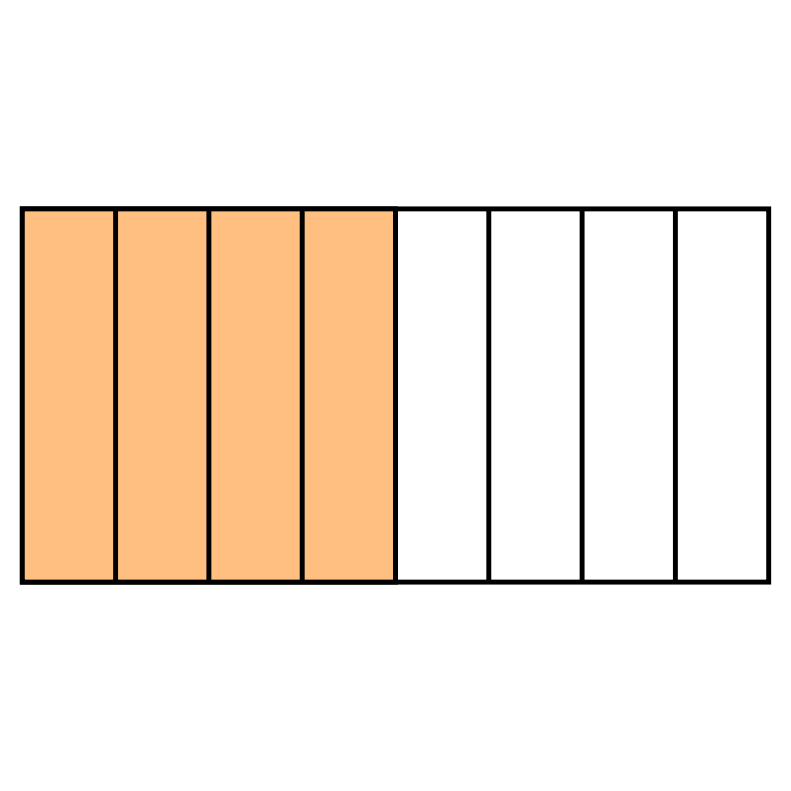
\includegraphics[width=60px]{../images/imagen_frac_5prim_4|8.png} \fillin[\fbox{$\dfrac{4}{8}$}][0in] \\[-0.5em]
			\part 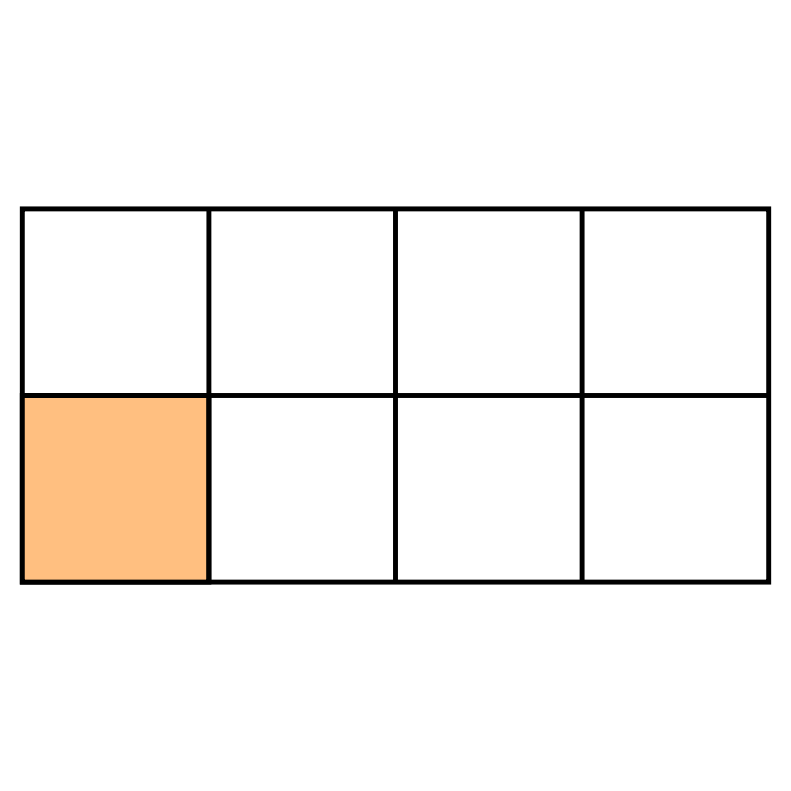
\includegraphics[width=60px]{../images/imagen_frac_5prim_1|8.png} \fillin[\fbox{$\dfrac{1}{8}$}][0in] \\[-0.5em]
			% \part 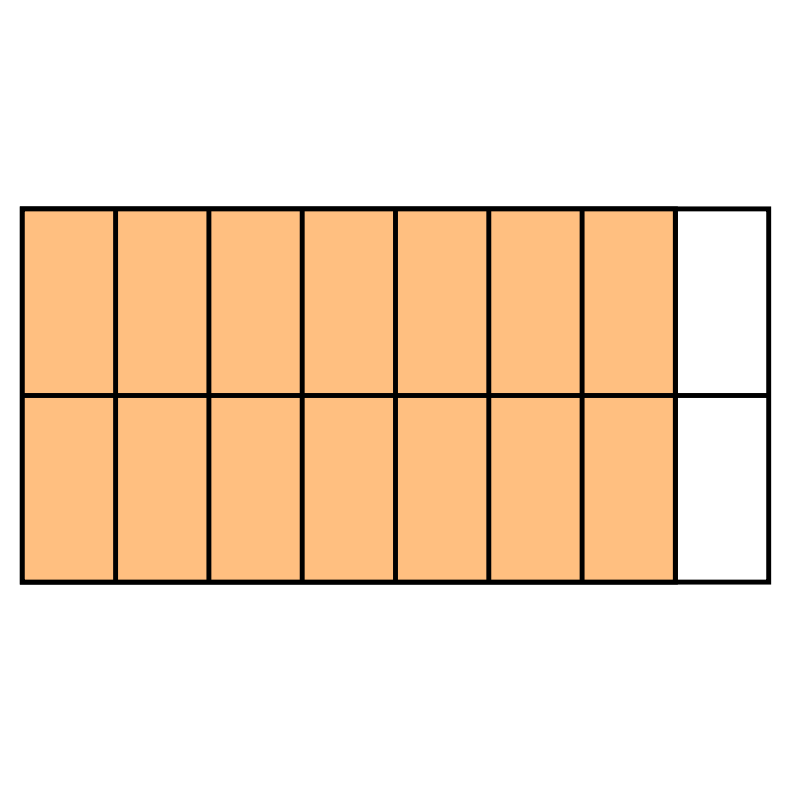
\includegraphics[width=60px]{../images/imagen_frac_5prim_14|16.png} \fillin[\fbox{$\dfrac{14}{16}$}][0in] \\[-0.5em]
			% \part 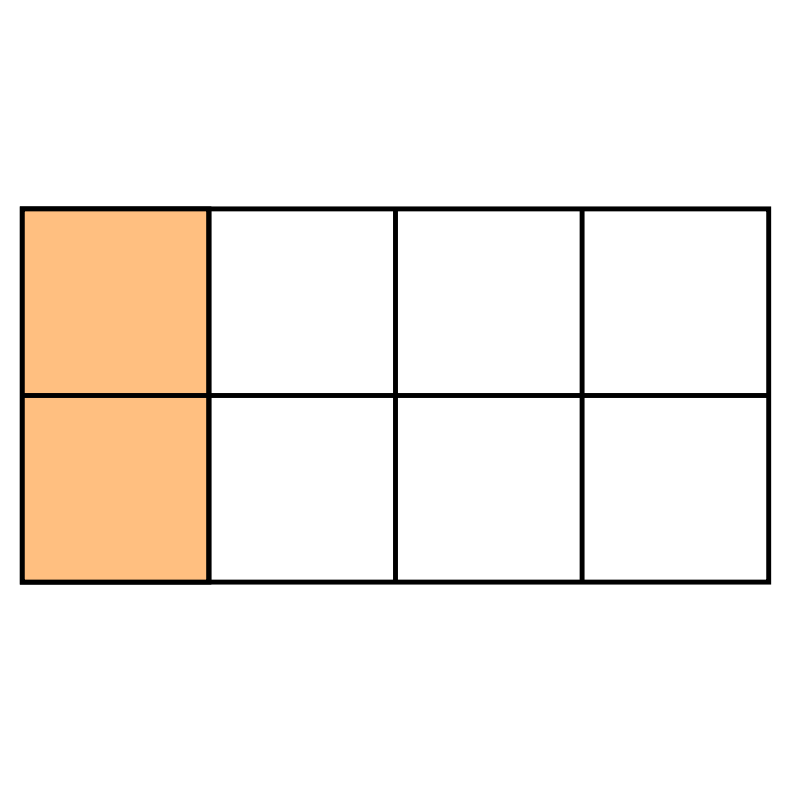
\includegraphics[width=60px]{../images/imagen_frac_5prim_2|8.png} \fillin[\fbox{$\dfrac{2}{8}$}][0in] \\[-0.5em]
			\part 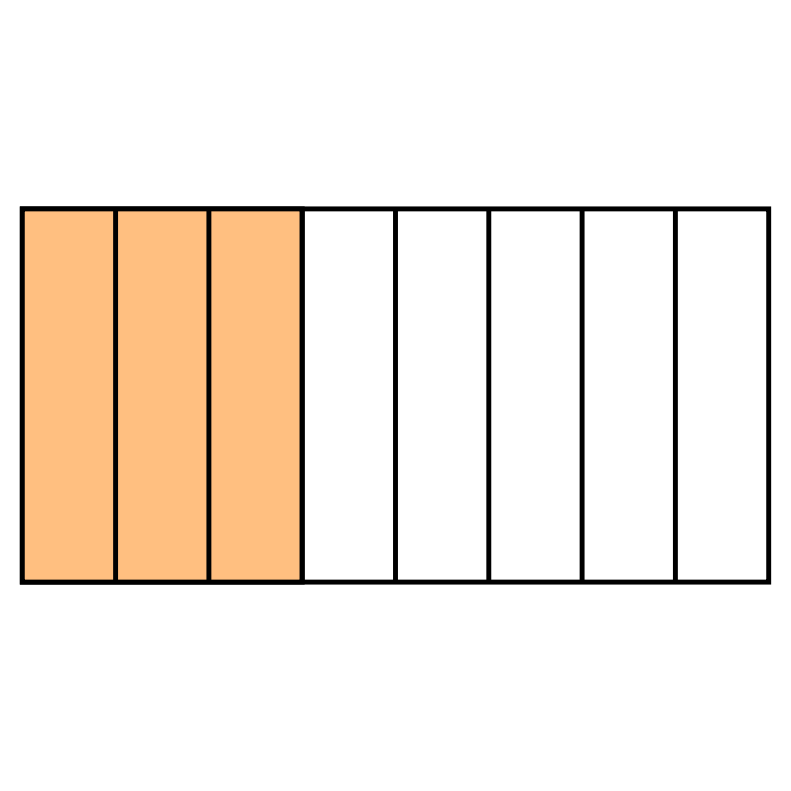
\includegraphics[width=60px]{../images/imagen_frac_5prim_3|8.png} \fillin[\fbox{$\dfrac{3}{8}$}][0in] \\[-0.5em]
			\part 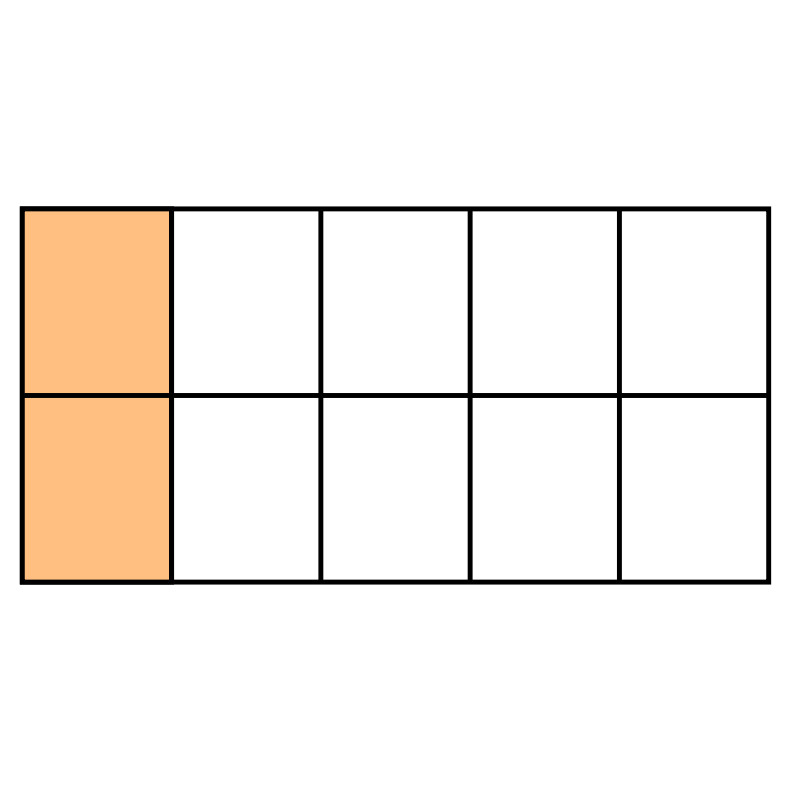
\includegraphics[width=60px]{../images/imagen_frac_5prim_2|10.png} \fillin[\fbox{$\dfrac{2}{10}$}][0in] \\[-0.5em]
			\part 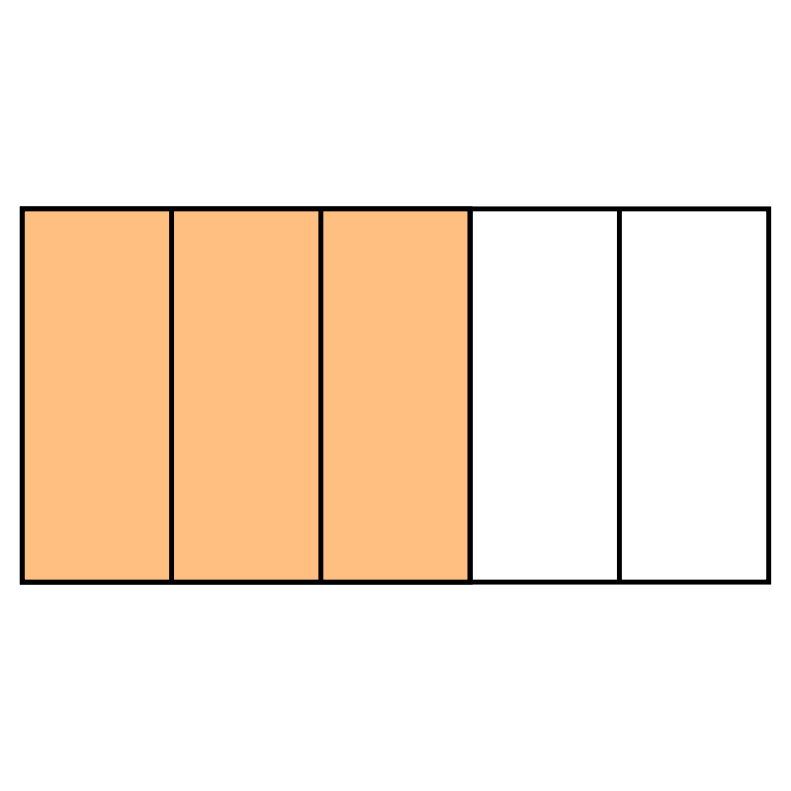
\includegraphics[width=60px]{../images/imagen_frac_5prim_3|5.png} \fillin[\fbox{$\dfrac{3}{5}$}][0in] \\[-0.5em]
			% \part 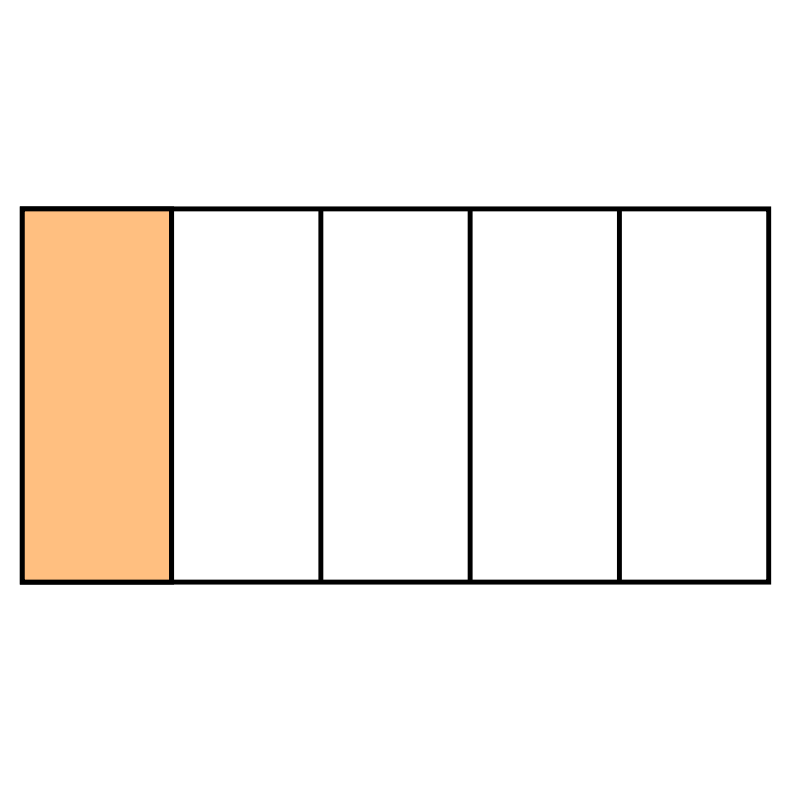
\includegraphics[width=60px]{../images/imagen_frac_5prim_1|5.png} \fillin[\fbox{$\dfrac{1}{5}$}][0in] \\[-0.5em]
			\part 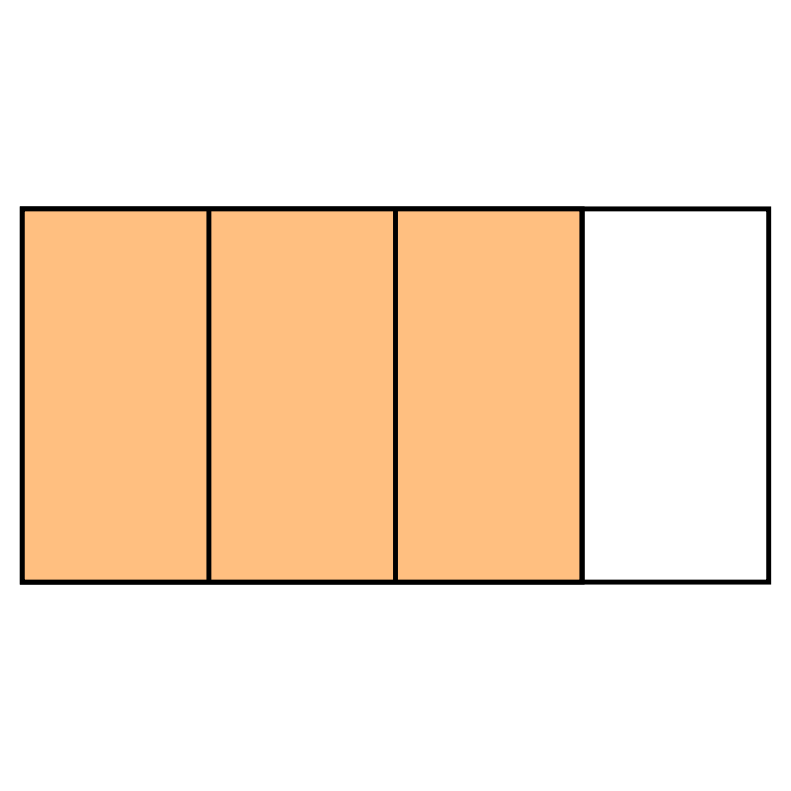
\includegraphics[width=60px]{../images/imagen_frac_5prim_3|4.png} \fillin[\fbox{$\dfrac{3}{4}$}][0in] \\[-0.5em]
		\end{parts}
	\end{multicols}
}

\question[6]{Escribe los siguientes porcentajes como números decimales:

	\begin{multicols}{3}
		\begin{parts}
			\part $14\%=$ \fillin[\fbox{0.14}][0cm]
			\part $73\%=$ \fillin[\fbox{0.73}][0cm]
			\part $15\%=$ \fillin[\fbox{0.15}][0cm]
			\part $85\%=$ \fillin[\fbox{0.85}][0cm]
			% \part $91\%=$ \fillin[\fbox{0.91}][0cm]
			% \part $19\%=$ \fillin[\fbox{0.19}][0cm]
			% \part $ 9\%=$ \fillin[\fbox{0.09}][0cm]
			\part $42\%=$ \fillin[\fbox{0.42}][0cm]
			\part $25\%=$ \fillin[\fbox{0.25}][0cm]
			% \part $ 3\%=$ \fillin[\fbox{0.03}][0cm]
			% \part $ 8\%=$ \fillin[\fbox{0.08}][0cm]
			% \part $ 2\%=$ \fillin[\fbox{0.02}][0cm]
		\end{parts}
	\end{multicols}
}


\question[10]{Resuelve los siguientes problemas sobre multiplicaciones:

	\begin{multicols}{2}
		\begin{parts}
			\part Una escuela tiene 6 salones, si cada salón tiene 25 alumnos. ¿Cuántos alumnos tiene en total la escuela?

			\begin{solutionbox}{1cm}
				\opmul[style=text]{6}{25}
			\end{solutionbox}

			% \part Una cubeta de pintura cuesta 2345 pesos, ¿cuánto se pagará por 3 cubetas de pintura?

			% \begin{solutionbox}{1cm}
			% 	\opmul[style=text]{3}{2345}
			% \end{solutionbox}

			% \part Una secretaria puede escribir 36 palabras por minuto si continua con este ritmo, ¿cuántas palabras puede escribir en 12 minutos?

			% \begin{solutionbox}{1cm}
			% 	\opmul[style=text]{36}{12}
			% \end{solutionbox}

			\part Cristina compró 5 cajas de leche de soya, si cada caja tiene 12 envases de leche, ¿cuántos envases de leche compró Cristina?

			\begin{solutionbox}{1cm}
				\opmul[style=text]{5}{12}
			\end{solutionbox}

			% \part Mariana fue a la frutería y compró 3 kilogramos de uvas, si el kilogramo cuesta 84 pesos. ¿Cuánto pagó en total Mariana?

			% \begin{solutionbox}{1cm}
			% 	\opmul[style=text]{3}{84}
			% \end{solutionbox}

			% \part Laura compró 28 paquetes de galletas, si cada paquete tiene 18 galletas. ¿Cuántas galletas tiene en total Laura?

			% \begin{solutionbox}{1cm}
			% 	\opmul[style=text]{28}{18}
			% \end{solutionbox}

		\end{parts}
	\end{multicols}
}

\question[8]{Selecciona la opci\'on que responde a cada una de las preguntas de forma correcta.

\begin{parts}
			\part ¿Cuál término describe al diagrama de la figura \ref{fig:act003a04}?

			\begin{minipage}{0.4\linewidth}
				\begin{figure}[H]
					\begin{center}
						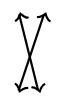
\includegraphics[width=0.2\textwidth]{../images/act003a04}
					\end{center}
					\caption{}
					\label{fig:act003a04}
				\end{figure}
			\end{minipage}
			\begin{minipage}{0.6\linewidth}
				\begin{choices}
					\choice Rectas paralelas.
					\choice Rectas perpendiculares.
					\choice Ninguna de las anteriores.
				\end{choices}
			\end{minipage}

			\part ¿Cuál término describe al diagrama de la figura \ref{fig:act003a08}?

			\begin{minipage}{0.4\linewidth}
				\begin{figure}[H]
					\begin{center}
						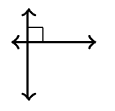
\includegraphics[width=0.3\textwidth]{../images/act003a08}
					\end{center}
					\caption{}
					\label{fig:act003a08}
				\end{figure}
			\end{minipage}
			\begin{minipage}{0.6\linewidth}
				\begin{choices}
					\choice Rectas paralelas.
					\choice Rectas perpendiculares.
					\choice Ninguna de las anteriores.
				\end{choices}
			\end{minipage}

			\part ¿Cuál de estos diagramas muestra rectas paralelas?
			\begin{multicols}{4}
				\begin{checkboxes}
					\choice 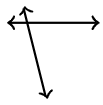
\includegraphics[width=0.1\textwidth]{../images/act003a10}
					\choice 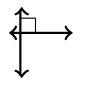
\includegraphics[width=0.1\textwidth]{../images/act003a06}
					\choice 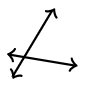
\includegraphics[width=0.1\textwidth]{../images/act003a07}
					\choice 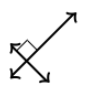
\includegraphics[width=0.1\textwidth]{../images/act003a09}
					% \choice 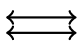
\includegraphics[width=0.1\textwidth]{../images/act003a05}
					% \choice 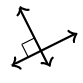
\includegraphics[width=0.1\textwidth]{../images/act003a11}
				\end{checkboxes}
			\end{multicols}


			\part ¿Cuál de estos diagramas muestra rectas perpendiculares?
			\begin{multicols}{4}
				\begin{checkboxes}
					% \choice 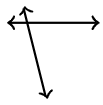
\includegraphics[width=0.1\textwidth]{../images/act003a10}
					\choice \includegraphics[width=0.1\textwidth]{../images/act003a06}
					% \choice \includegraphics[width=0.1\textwidth]{../images/act003a07}
					\choice \includegraphics[width=0.1\textwidth]{../images/act003a09}
					\choice \includegraphics[width=0.1\textwidth]{../images/act003a05}
					\choice \includegraphics[width=0.1\textwidth]{../images/act003a11}
				\end{checkboxes}
			\end{multicols}


		\end{parts}

}

\end{questions}
\end{document}